% -----------------------------------------------
% Template for SMAC SMC 2013
% adapted and corrected from the template for SMC 2012, which was adapted from that of SMC 2011
% further updated for TENOR 2015, 2016, 2017 and 2018
% -----------------------------------------------

\documentclass{article}
\usepackage{tenor}
\usepackage{ifpdf}
\usepackage[english]{babel}
\usepackage{balance}

\input{js-code-format}
\input{json-format}
%\usepackage{listings}


%%%%%%%%%%%%%%%%%%%%%%%% Some useful packages %%%%%%%%%%%%%%%%%%%%%%%%%%%%%%%
%%%%%%%%%%%%%%%%%%%%%%%% See related documentation %%%%%%%%%%%%%%%%%%%%%%%%%%
%\usepackage{amsmath} % popular packages from Am. Math. Soc. Please use the 
%\usepackage{amssymb} % related math environments (split, subequation, cases,
%\usepackage{amsfonts}% multline, etc.)
%\usepackage{bm}      % Bold Math package, defines the command \bf{}
%\usepackage{paralist}% extended list environments
%%subfig.sty is the modern replacement for subfigure.sty. However, subfig.sty 
%%requires and automatically loads caption.sty which overrides class handling 
%%of captions. To prevent this problem, preload caption.sty with caption=false 
%\usepackage[caption=false]{caption}
%\usepackage[font=footnotesize]{subfig}


\def\papertitle{Symbolist Re-imagined: bidirectional graphic-semantic mapping for media notation authoring and performance}
\def\firstauthor{Rama Gottfried} 
\def\copyrightyear{2022}


\usepackage{xspace}
\def\symbolist{\textsc{symbolist}\xspace}
\def\drawsocket{\textsc{drawsocket}\xspace}
\def\uicontroller{ui-controller\xspace}
\def\iocontroller{io-controller\xspace}
\def\uiapiFunction{\textit{ui\_api}}
\def\uiapi{\textit{ui\_api}\xspace}
\def\ioapiFunction{\textit{io\_api}}
\def\ioapi{\textit{io\_api}\xspace}
\makeatletter
\newcommand{\verbatimfont}[1]{\renewcommand{\verbatim@font}{\ttfamily#1}}
\makeatother


%% Depending on the number of authors, set this variable accordingly for the copyright notice:
\def\copyrightauthor{Rama Gottfried}

\def\oscfontsize{\tiny}


% pdf-tex settings: detect automatically if run by latex or pdflatex
\newif\ifpdf
\ifx\pdfoutput\relax
\else
   \ifcase\pdfoutput
      \pdffalse
   \else
      \pdftrue
\fi

\ifpdf % compiling with pdflatex
  \usepackage[pdftex,
    pdftitle={\papertitle},
    pdfauthor={\firstauthor},
    bookmarksnumbered, % use section numbers with bookmarks
    pdfstartview=XYZ % start with zoom=100% instead of full screen; 
                     % especially useful if working with a big screen :-)
   ]{hyperref}
  %\pdfcompresslevel=9

  \usepackage[pdftex]{graphicx}
  % declare the path(s) where your graphic files are and their extensions so 
  %you won't have to specify these with every instance of \includegraphics
  \graphicspath{{./figures/}}
  \DeclareGraphicsExtensions{.pdf,.jpeg,.png}

  \usepackage[figure,table]{hypcap}

\else % compiling with latex
  \usepackage[dvips,
    bookmarksnumbered, % use section numbers with bookmarks
    pdfstartview=XYZ % start with zoom=100% instead of full screen
  ]{hyperref}  % hyperrefs are active in the pdf file after conversion

  \usepackage[dvips]{epsfig,graphicx}
  % declare the path(s) where your graphic files are and their extensions so 
  %you won't have to specify these with every instance of \includegraphics
  \graphicspath{{./figures/}}
  \DeclareGraphicsExtensions{.eps}

  \usepackage[figure,table]{hypcap}
\fi

%setup the hyperref package - make the links black without a surrounding frame
\hypersetup{
    colorlinks,%
    citecolor=black,%
    filecolor=black,%
    linkcolor=black,%
    urlcolor=black
}


% Title.
% ------
\title{\papertitle}

\oneauthor
   {\firstauthor} { Hochschule für Musik und Theater \\ Hamburg, Germany \\
     {\tt \href{mailto:rama.gottfried@hfmt-hamburg.de}{rama.gottfried@hfmt-hamburg.de}}}



% ***************************************** the document starts here ***************
\begin{document}
%
\capstartfalse
\maketitle
\capstarttrue


\begin{abstract}

\symbolist is an in-development application for experimental notation, which aims to provide an un-opinionated authoring environment for the design and performance of symbolic notation. 
By following an information visualization rather than prescribed musical orientation, the application is thought of as an open play-space, with tools for experimentation and thinking visually about relationships between representation and interpretation in media performance.
In the paper we begin with an overview of the project's background, iterations and relationship to the \drawsocket project, and introduce a redesign of the system, centered on a new framework for custom symbol definitions for bidirectional mapping and user interaction.
In conclusion we discuss future development directions and evaluation of the project.

\end{abstract}


\section{Background}\label{sec:background}

The origins of the \symbolist project can be traced back to 2011, through the development of a composition practice in Adobe Illustrator using a plugin called Scriptographer,\footnote{https://scriptographer.org/} which allowed users to create new drawing tools in Javascript which could then be used in Illustrator as an interactive brush. 
As a composer working with experimental instrumental techniques and spatial notation, Scriptographer was perfect for my composition needs at the time, since you could design a notation for a given technique or musical expression and then code it as an interactive graphic function, which could then be manipulated graphically in Illustrator. 
With the access to the mouse movement, interactions could be used to compose different elements of the notation, much in the same way that mouse interaction is used in programs like Processing.\footnote{https://processing.org/}

For example, a note with a spatially indicated duration typically is written as a note-head of some shape with a line extending out from it to show its duration. 
Using Scriptographer, you could create an interaction for composing note-duration symbols, where clicking down on the Illustrator canvas places the note-head, and then using the mouse drag, determine the end of the duration line, ending at the location of the mouse up event.

Further, you could also group elements to structure hierarchies of objects which would then appear in Illustrator as grouped objects, visible as nested folders in the layers menu.

%Scriptographer's drawing API provided a set of basic vector primitives and grouping methods that closely parallel the objects found in Scalable Vector Graphics (SVG) format~\footnote{https://www.w3.org/TR/SVG11} which is well supported in Adobe Illustrator. 

Around the same time, I was studying at UC Berkeley's Center for New Music and Audio Technologies (CNMAT) developing approaches to instrument design using OpenSoundControl (OSC)~\cite{wright:osc} for data structuring. 
One day, while working with Scriptographer, I had saved a score in Illustrator as Scalable Vector Graphics (SVG) format~\footnote{https://www.w3.org/TR/SVG11} and accidentally opened the SVG file in a text editor. 
In the SVG file I noticed that all of the graphic objects were there in a human readable format, and closely resembled the kind of nested objects that we were working on at CNMAT in the Odot library\cite{maccallum2015dynamic}. This gave me the idea that I might be able to translate the SVG information into OSC, then ``perform'' the OSC score in much the same way as you would a stream of OSC coming from a sensor-based instrument—in a similar spirit to Daphne Oram's ``Oramics''~\cite{manning2012oramics} and Xenakis' UPIC system~\cite{marino1993upic}, but with a greater focus on symbolic interpretation. 
%The first tests seemed promising, and so I logged it away for possible future use.

Soon after, while composing for a high-resolution spatial audio rendering system, I found that I was lacking a way to compose spatial movements graphically, in a way that would connect with instrumental notation practice.
After some experiments using Blender\footnote{https://www.blender.org/} to draw 3D curves which could then be parsed via Python and sent out over OSC, I was dissatisfied by the perceptual differences between common practice notation and the kinds of 3D representation I was able to create in Blender—both had their merits, but what was missing was a compositional frame that connected the two representation paradigms into a unified notation system.
Due to time constraints, for this piece I fell back on using automation controls in Ableton Live\footnote{https://www.ableton.com/en/} and sending OSC to control the movements using Max for Live.\footnote{https://cycling74.com/}
This was practical, but this kind of automation approach has the limitation of forcing the composer to separate each data parameter into separate streams of data (e.g. $x, y, z$), whereas in a symbolic representation multiple attributes can be indicated in unified graphic representation. 
Following these experiences~\cite{gottfried2013studies} I later returned to the SVG-OSC transcoding idea, and developed a first working model which was presented at the 2015 TENOR conference~\cite{gottfried2015svg}.

In the meantime, the Scriptographer project was abandoned by its developers after Adobe drastically changed their plugin API in version CS6. 
The new Adobe API was different enough that it would require a significant amount of work, and even then the mouse interaction tools that were used in Scriptographer were no longer accessible, so the authors decided to stop development on the project and later went on to create Paper.js,\footnote{http://paperjs.org/} which has some similarities with Scriptographer, but is more closely related to Processing since it no longer is bound to the Illustrator application environment. 

%This created a stumbling block for the SVG-OSC work, since it relied on Scriptographer and its link to Illustrator as primary tools for the creation of easy to print scores for musicians to perform with. 

\subsection*{Symbolist JUCE}\label{sec:juce_version}

After preliminary tests using the SVG-OSC transcoding for score playback, it was becoming increasingly complicated to parse complex hierarchies of symbols in order to format them into OSC streams, so in 2017 I began work in collaboration with OpenMusic~\cite{bresson2011om} developer Jean Bresson, through an Ircam-ZKM Musical Research Residency towards the goal of creating a system that could replace the Scriptographer/Illustrator approach that I had developed so far.

The first version of \symbolist was created in 2018 as a standalone JUCE\footnote{https://juce.com/} application, which provided the basic tools for drawing vector graphics and query system that allowed \symbolist to be used as a lookup table for OSC stream playback~\cite{gottfried2018symbolist}.

Working in JUCE seemed practical since it has a wide user base and is used for audio plugins as well as Max and Ableton Live applications.
There were some minor complications, due to JUCE's incomplete SVG support,\footnote{https://forum.juce.com/t/complex-svg-files-fail-to-load-properly/26917/16} however, generally, we were able to create a working first prototype of the system.

\subsection*{Clefs and Bidirectional Mapping}\label{sec:bidirectional_mapping}

A conceptual turning point in the project occurred towards the end of the residency as we were thinking about how to simplify the process of using the SVG data for controlling digital processes.

In the first version of \symbolist, as in the original SVG-OSC implementation, the graphic data needed to be interpreted by the application that received the data. 
Using Odot I would parse the graphic OSC information coming in from \symbolist, and then map the data to other processes, for instance synthesis parameters or coordinates for spatial rendering. 

The process of interpretation requires that the parsing-mapping algorithm knows the context of the graphic objects. For example, that a circle is a note-head and not a rhythmic dot, and so on. 
Like the axes of a graphic plot of information, contextual musical symbols (meter, staff-lines, clefs) indicate to the reader how they should interpret the notes and rhythmic symbols written on the staff.

The following phase of \symbolist development continued as I began work at the Hamburg University of Music and Theater, working with Georg Hajdu in the Innovative Hochschule project. 
Continuing from the idea of the \textit{clef} as a graphic symbol that contextualizes the notation on a musical staff, I began work on developing a system for \symbolist that would allow users to define interpretive symbols for hierarchical context parsing.
Since the data is already in hierarchical format inside the application's data structure, it was logical that \symbolist could interpret the graphics internally, and then stream OSC post parsing and mapping, rather than streaming the raw graphic information which required complex parsing of the graphic hierarchies to contextualize the symbol references, as in traditional common practice notation.

Following this line of thought it became clear that what \symbolist really needed was a system for \textit{bidirectional mapping}, where graphic data is interpreted as symbolic data with semantic meaning, and inversely, that the user should also be able to send data in its semantic representation to \symbolist, where it would then be mapped to its graphic representation.

In 2018 I began implementing this idea into the JUCE version of \symbolist, but soon needed to switch tracks to focus on a different notation issue for a project at the Innovative Hochschule, developing a platform for realtime networked score display.

\subsection*{Drawsocket and Symbolist JS}\label{sec:drawsocket}

At the end of 2018, and first half of 2019 we developed a drawsocket, a server/client framework for realtime dynamic notation using web browsers for graphic rendering~\cite{gottfried2019drawsocket, hajdu2005quintet}. 
Based in node.js and standard web technologies of HTML, SVG, CSS, and Javascript, \drawsocket is essentially an OSC wrapper~\cite{freed2014io} for web browsers,\footnote{And by extension, provides access to other media via WebAudio, WebGL, etc.} providing a homogeneous message API for the creation and realtime manipulation of browser elements.

Returning to \symbolist after the first \drawsocket concerts, I began wondering if the framework of \symbolist needed to be redesigned from the perspective of bidirectional mapping, since I realized that this was most likely going to be the most important part of the graphic-data relationship that the system is developing towards. 

SVG is very well supported in modern browsers, and having just worked with node.js and browser technologies for \drawsocket, it seemed that the flexibility of Javascript could be a convenient option for users to create custom symbol definitions (as in Scriptographer). I decided to see how fast it would be to implement a proof of concept using Electron.js,\footnote{https://www.electronjs.org/} a cross-platform desktop application development using a node.js server and Chrome as a front-end, used for applications like Skype, WhatsApp, Visual Studio Code, Slack, WordPress, and others.
%While developing \drawsocket, I did some study into frameworks such like React\footnote{https://reactjs.org/} which provide object oriented ways of handling graphic interfaces, not unlike the approaches used in JUCE, however after working in JUCE, I wanted something lightweight and simple to start with.

Using \drawsocket as a frontend, and node.js for the backend I found that I was able to get up and running very quickly with Electron, and decided to continue \symbolist development in this direction, bringing the experience gained from the JUCE version to the creation of a deeper structure for the creation of symbol interpretations that integrate into the graphic manipulation of symbolic data. 

% screenshot
\begin{figure*}[hbt!]
\centering
\includegraphics[width=2\columnwidth]{symbolist.png}
\caption{ \symbolist screenshot, showing some different types of staves, and editing capabilities.
\label{fig:screenshot}}
\end{figure*}


%% Implementations
%\section{Implementation}\label{sec:implementations}
%
%Electron\footnote{https://www.electronjs.org/} version (node + chrome w/ special electron IPC)
%Max version (node + jweb + Max patch for IPC)


\begin{figure*}[hbt!]
\centering
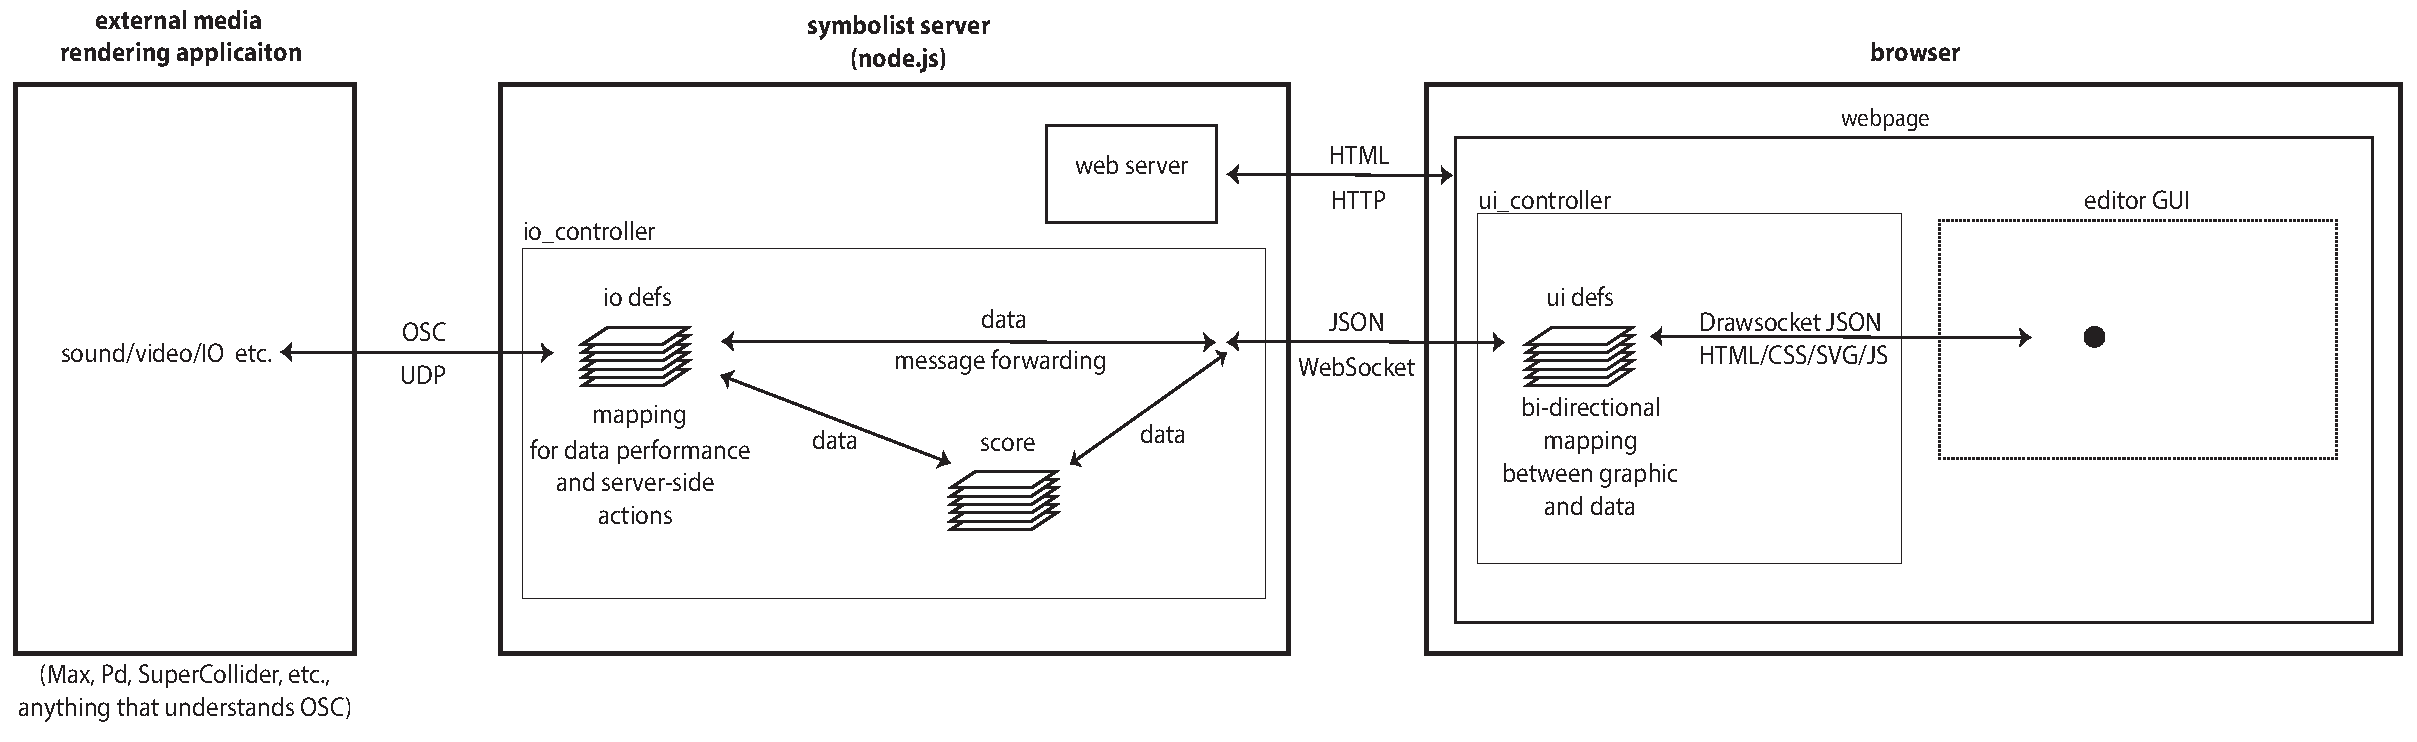
\includegraphics[width=2\columnwidth]{symbolist-architecture2.pdf}
\caption{ \symbolist architecture.
\label{fig:architecture}}
\end{figure*}

% Application Structure
\section{Application Structure}\label{sec:application_structure}

The new implementation of \symbolist is organized as a server-client model (Figure~\ref{fig:architecture}), comprising of:

\begin{itemize}\itemsep0pt 

\item The main \symbolist application server, running in node.js, which serves the main display page and manages messages between the client and server via WebSocket\footnote{https://websockets.spec.whatwg.org} connection. 
Within the main server, a child process called the ``\iocontroller''  handles input and output from external sources via OSC over a UDP socket, and maintains the ``\textit{score},'' a database of hierarchical score elements, stored in \symbolist ``\textit{semantic representation}'' format (Section \ref{sec:representation}).

\item The ``\textit{editor},'' a browser-based user interface client, which displays the graphic representation of the data, and allows the user to edit and create new data objects through graphic interaction. The ``\uicontroller'' runs in the browser and handles interaction via a library of definition scripts, which specify mappings to and from data and graphics formats, as well as other tools and interactions.


\end{itemize}

Since the system is now based on a web-server model, we are able to also use Max's \textit{node.script} object to run the server from within Max as an alternative to the Electron desktop app.
%The \iocontroller holds a copy of the score in its semantic data format (described below), and loads a library of user scripts shared with the \uicontroller which define the mapping to (and potentially from) other media sources. 
%
%The \iocontroller can also be used to translate the score into other formats that can be performed by another sequencing tool or program like MaxMSP.
%

\section{Graphical Authoring and Interaction}\label{sec:editor} 

The \symbolist graphic user interface (Figure~\ref{fig:screenshot}) is designed around units of symbolic objects and their contextual containers.
Graphic ``\textit{symbol}'' objects are placed in ``\textit{container}'' symbols, which function as a context frame that can be used to interpret the meaning of the symbol.

In order to maintain an open and un-opinionated approach, the \symbolist framework does not specify how containers and symbols should look, act, or respond when you interact with them. 
Rather, the interaction and meanings of the symbols are defined in a library of custom object ``\textit{definitions},'' which specify meaning through mapping semantic data to-and-from its graphic representation. 

Symbol definitions provide a mechanism to design custom-tailored composition environments for particular authoring situations, stored as Javascript libraries, which can be shared between users, and used as templates.
Leveraging web-browser technologies like JS, HTML, CSS, SVG, etc., there are many ways to customize the layout in \symbolist, and potentially, the definition libraries could completely transform the editor layout to serve a particular use-case scenario.

\subsection*{Interface Components}\label{sec:interface_components}

%The default \symbolist graphic editor (Figure~\ref{fig:screenshot}) provides the basic mechanisms for user interaction, to create scores through the creation of hierarchical object relationships.
The main graphic components of the default \symbolist graphic editor are:

\begin{itemize}\itemsep0pt 
\item 
\textit{Score view}: the top-level view of the application window, containing the main view and side bar. Sliders are provided to offset the view of the document, as well as basic zoom functionality.
\item 
\textit{Palette}: a set of buttons in a side toolbar displaying icons of symbols that have been defined for the current selected container context. 
\item 
\textit{Tools}: a set of buttons that open high-level tools, that can be used for operations like algorithmic generation of new symbols, or applying transformations to existing elements (e.g. alignment of multiple objects, setting distributing objects, or other operations).
\item 
\textit{Inspector}: a contextual menu for editing the semantic data of a selected symbol, which on update is mapped to the graphic representation and sent to the server to update the main score database.
%\item 
%\textit{Menu bar}: the menu bar at the top of the screen or window, which provides access to various application functions.
\end{itemize}
%
%\subsection{Modes}\label{sec:modes}
%
%In the \symbolist workflow, the user shifts between different modes, each of which has user-definable behaviors in the definitions library.
%The current modes are:
%\begin{itemize}\itemsep0pt 
%\item \textit{Palette}: clicking on an icon in the palette sidebar enables the user interaction assigned to the clicked symbol type.
%\item \textit{Creation}: holding down the CMD key (Mac) enters \textit{creation mode}, telling \symbolist to create a new \textit{symbol} of the type selected in the palette, similarly this action may enable different types of user interaction, for example snapping the symbol to specified pixels, etc.
%\item \textit{Selection}: clicking on a pre-existing \textit{symbol} in the document will \textit{select} the object, which notifies a callback in the definition script for possible interaction.
%\item \textit{Edit}: if a user has selected an object and then types the letter [e], \symbolist will attempt to enter \textit{edit mode} if there is one defined in the symbol definition script. This is useful for example in the case of a bezier curve; entering \textit{edit mode} could make visible the handles for the curve for editing.
%\item \textit{Inspector}: if a user has selected an object and then types the letter [i], an inspector window appears showing the \textit{semantic data} corresponding to the symbol's graphical information (datatypes are discussed further in section~\ref{sec:representation} below).
%\end{itemize}
%
\subsection*{User Experience}\label{sec:ux}

On entering the application, the editor loads a score or configuration file from the default load folder, which sets the top-level page setup and palette options. A typical sequence of creating a score might be as follows:
\begin{enumerate}\itemsep0pt
\item The user opens a workspace with one or more default container symbols displayed on the screen, for example an empty rectangle, which is like a piece of paper.
\item Clicking on the ``paper'' container rectangle \textit{selects} it, and then the user sets it as the new \textit{context} by pressing the [s] key.
\item After setting the context, the palette toolbar is populated with icons of symbols that are defined with the selected container context type.
\item Clicking on one of the palette toolbar symbol icons puts the interface into ``\textit{palette mode},'' where the mouse interaction is now designed for use with this specific symbol type.
\item Holding the Command(Mac)/Control(Win) key enters ``\textit{creation mode},'' which by convention draws a temporary preview of the symbol (how it will appear when you click), and displays the corresponding semantic representation data as textual feedback.
\item After clicking, the symbol is placed in the container.
\item Clicking and dragging a symbol graphically modifies its semantic data in reference to the container context. In the case of common practice notation this would be how you would change the time and pitch information of a symbol. The interaction results depend on the ``\textit{selection mode}'' specified in the symbol definition.
\item User can also modify the semantic parameters as text by selecting the symbol and hitting the [i] key, which brings up the inspector window, where you can edit the data directly.
\item Pressing the [e] key enters ``\textit{edit mode}'' for the selected symbol, useful for editing of internal attributes that are less relative to the container symbol. For example, you would enter edit mode to adjust bezier curve anchor points.
\end{enumerate}

\section{Data Representation}\label{sec:representation}

At the heart of \symbolist are two parallel forms of information expression: \textit{semantic} and \textit{graphic} representation (Figure~\ref{fig:graphic-representation}).

\textit{Semantic} data specifies the various attributes of information about a symbolic object in terms of the object's meaning to the author. 
For example, the meaningful attributes of a \textit{note} object might be information about pitch and duration, or a \textit{point} object might contain x, y, and z values corresponding to the point's location in 3D space. 
In \symbolist the semantic representation is thought of as the main holder of information, which can be grouped into hierarchies to represent scores or other types of data structures.

The \textit{graphic} representation is a symbolic visual expression of the semantic data, designed relative to the context defined by the author. 

The aim of \symbolist is to provide an agnostic environment for developing, and composing with, new symbolic representations of semantic data for use in multimedia composition practice; and so, the central design consideration of this new implementation is to build a flexible framework for specifying a wide range of mapping relationships between semantic and graphic representations.

\begin{figure}[ht!]
\centering
\includegraphics[width=1\columnwidth]{graphic-representation.pdf}
\caption{\textit{Semantic} vs \textit{graphic} representation of the same information. Note: Figures \ref{fig:graphic-representation}-\ref{fig:score-lookup} use pseudocode for brevity (see Sections \ref{sec:semantic} and \ref{sec:graphic_display_format} for  syntax details).
\label{fig:graphic-representation}}
\end{figure}


\section{Mapping}\label{sec:mapping}

Between each of these representation contexts there is a layer of mapping, with the \textit{semantic data} serving as the primary representation type. 

\textit{Semantic data to graphic representation} mapping (Figure~\ref{fig:data-to-graphic}) is used for the creation of graphic symbols from a stream of input, for example from generative processes, textural authoring, or computer assisted composition systems~\cite{bresson2011om, didkovsky2008maxscore, agostini2015max, baca2015abjad, burloiu2017visual}.

\textit{Graphic representation to semantic data} mapping (Figure~\ref{fig:graphic-to-data}) is used in order to create or edit data based on graphic information. This is the typical ``graphical user interface'' situation, where the data is accessible through its visual representation.

\textit{Semantic data to performance media} mapping (Figure~\ref{fig:score-lookup}) is the use of the data as a sequence of events that can be played in time (or used to control other processes not necessarily in time).

Note that in \symbolist mapping between \textit{performance media} and \textit{graphic representation} is achieved through first mapping to semantic data. See section~\ref{library_definitions_api} for further discussion.


% mapping figures

\begin{figure}[ht!]
\centering
\includegraphics[width=0.9\columnwidth]{data-to-graphic.pdf}
\caption{\textit{Semantic} data mapped to create a \textit{graphic} representation from input data. 
\label{fig:data-to-graphic}}
\end{figure}

\begin{figure}[ht!]
\centering
\includegraphics[width=0.9\columnwidth]{graphic-to-data.pdf}
\caption{If edited graphically, the updated graphic data is then mapped back to \textit{semantic data} representation. 
\label{fig:graphic-to-data}}
\end{figure}

\begin{figure}[ht!]
\centering
\includegraphics[width=1\columnwidth]{score-lookup.pdf}
\caption{Using the lookup method defined by the symbol class, the \textit{semantic data} can be used to perform external instruments via Open Sound Control. 
\label{fig:score-lookup}}
\end{figure}



%
%\section{Symbols}\label{sec:symbols}
%
%In \symbolist terminology, a ``\textit{symbol}'' is object that connects the semantic and graphic aspects together as a multifaceted unit.
%Each \textit{symbol} is defined as a \textit{class} of object, which specifies the symbol's data structure and UI interaction, and data mapping to different representational contexts.

\section{Semantic Representation}\label{sec:semantic}

Within the \symbolist application semantic data is stored as Javascript objects and read/written in JSON\footnote{https://www.json.org/json-en.html} format (transcoded to-and-from OSC for inter-application communication).

The main attributes used in \symbolist semantic data objects are:

\begin{itemize}\itemsep0pt 
\item \textit{id}: a unique identifier name (required).
\item \textit{class}: a reference to the definition of the object type in the user-definition library (required).
\item \textit{contents}: an array of child objects that a parent container object might hold (required for container symbols).
\end{itemize}

Semantic data objects may include any number of other attributes\footnote{The term \textit{attribute} is used here interchangeably with properties, parameters, aspects, etc.} (\textit{pitch}, \textit{amplitude}, etc.). 
For example a simple semantic object might look like:

\begin{lstlisting}[
belowskip=-2 \baselineskip,
 language=Javascript,
  mathescape,
  columns=fullflexible,
  breaklines=true,
  basicstyle=\oscfontsize\fontfamily{lmvtt}\selectfont,
]
{
    "id" : "foo",
    "class" : "legs",
    "action" : "jump",
    "start_time" : 0.1
}
\end{lstlisting}

\noindent
Here we see an object with the \textit{id} ``foo,'' which is of \textit{class} ``legs,'' that has an attribute \textit{action} associated with it and a start time.

\subsection*{Containers}
Symbols may also contain other symbols. 
Container symbols function to frame their contents, providing reference and context like a plot graph frame, which provides a perspective and scaling for interpreting the set of data points displayed in the graph.
Similarly, when a semantic data object contains other objects, the children are stored as an array in the object's \textit{contents} field. For example, for an imaginary class ``timeline,'' which holds two types of leg actions, we might write:

\begin{lstlisting}[
belowskip=-2 \baselineskip,
 language=Javascript,
  mathescape,
  columns=fullflexible,
  breaklines=true,
  basicstyle=\oscfontsize\fontfamily{lmvtt}\selectfont,
]
{
    "id" : "bar",
    "class" : "timeline",
    "duration" : 1,
    "contents" : [{
        "id" : "foo-1",
        "class" : "legs",
        "action" : "jump",
        "start_time" : 0.1
    },{
        "id" : "foo-2",
        "class" : "legs",
        "action" : "sit",
        "start_time" : 0.2
    }]
}

\end{lstlisting}

% move this to the definitions discussion? (already there I think)
%In most cases, a symbol's mapping definition will require querying its parent symbol for information, in order to plot its data relative to the container context, for example offsetting the screen coordinate position based on the parent object position.

\subsection*{Score Files}\label{sec:score}

%Using objects and container objects, we can form tree structures to represent hierarchical grouping.
%At the root of the tree structure is a top-level object, which might (but not necessarily) define behavior of its children objects.

Since the data elements are stored as JS objects, it is easy to import/export \symbolist scores as JSON files.

When the application loads, it reads a default initialization file in the form of a \symbolist score.
The current default initialization config file looks like this:

\begin{minipage}{\linewidth}
\begin{lstlisting}[
belowskip=-2 \baselineskip,
 language=Javascript,
  mathescape,
  columns=fullflexible,
  breaklines=true,
  basicstyle=\oscfontsize\fontfamily{lmvtt}\selectfont,
]
{
    "about" : "some metatdata",
    "id" : "Score",
    "class" : "RootSymbol",
    "contents": { 
        "id" : "trio",
        "class" : "SystemContainer",
        "x": 200,
        "y": 100,
        "duration": 20,
        "time": 0,
        "contents" : [{
            "id" : "oboe",
            "class" : "FiveLineStave",
            "height" : 100,
            "duration": 20,
            "time": 0,
            "contents" : []
        },
        {
            "id" : "bassoon",
            "class" : "PartStave",
            "height" : 100,
            "time": 0,
            "duration": 20,
            "contents" : []
        },
        {
            "id" : "synth",
            "class" : "PartStave",
            "height" : 200,
            "time": 0,
            "duration": 20,
            "contents" : []
        }]
    }
}
\end{lstlisting}
\end{minipage}

In this example, we can see there is a ``RootSymbol,'' which contains a ``SystemContainer,'' which in turn contains two ``PartStave'' symbols and one ``FiveLineStave'' symbols.

\section{Browser Notation}\label{sec:graphic_display_format}

\symbolist uses SVG to draw graphic symbol representation, utilizing \drawsocket as a convenience wrapper to provide shorthand methods to create and manipulate browser window elements. 

\subsection*{SVG / HTML Format}

The \symbolist format for a \textit{symbol} in its browser-rendered notation, is a set of three group elements ($<$g$>$ in SVG, or $<$div$>$ in HTML) marked by \textit{class} tags, which follow the defined symbol class name.

For a symbol class type ``SymbolClassName,'' the SVG template would be:

\begin{lstlisting}[
belowskip=-2 \baselineskip,
 language=Javascript,
mathescape, columns=fullflexible, breaklines=true,basicstyle=\oscfontsize\fontfamily{lmvtt}\selectfont]
<g  id="foo" class="SymbolClassName symbol">
    <g class="SymbolClassName display"></g>
    <g class="SymbolClassName contents"></g>
</g>
\end{lstlisting}

The ``\textit{symbol}'' class marks the top-level symbol group containing the ``\textit{display}'' and ``\textit{contents}'' groups. The ``\textit{display}'' group holds all of the symbol's display information and the ``\textit{contents}'' group contains any potential child elements. 
For simplicity all graphic \textit{symbol} elements include both the \textit{display} and \textit{contents} elements as placeholders.

%Symbols and containers can also be HTML elements instead of SVG. In the case of HTML you would use $<$div$>$ instead of $<$g$>$ tags for the symbol elements.

%\begin{lstlisting}[
%belowskip=-2 \baselineskip,
% language=Javascript,
%  mathescape,
%  columns=fullflexible,
%  basicstyle=\oscfontsize\fontfamily{lmvtt}\selectfont,
%]
%<div id="bar" class="SymbolClassName symbol">
%    <div class="SymbolClassName display"></div>
%    <div class="SymbolClassName contents"></div>
%</div>
%\end{lstlisting}


\subsection*{Storing Semantic Data in Dataset Attributes}\label{sec:dataset}

Since \symbolist is constantly mapping back and forth between semantic data and its graphic representation, we are making use of the HTML \textit{dataset} feature\footnote{https://developer.mozilla.org/en-US/docs/Web/API/HTMLElement/dataset} to store the semantic metadata inside the top-level \textit{symbol} element.

For example, using our imaginary ``legs'' actions above, we include the \textit{action} and \textit{start\_time} parameters, written as dataset attributes by using the prefix ``\textit{data-}'':\footnote{Note that according to the HTML dataset specifications, all names will be converted to lowercase, this can create issues in some cases, so best practice is to use all lowercase for attribute names.}

\begin{minipage}{\linewidth}
\begin{lstlisting}[language=Javascript,
belowskip=-2 \baselineskip,
%float=*,
mathescape, columns=fullflexible, breaklines=true,basicstyle=\oscfontsize\fontfamily{lmvtt}\selectfont]
<g  id="bar" class="Timeline symbol" 
							data-duration="1">
  <g class="Timeline display"></g>
  <g class="Timeline contents">
      <g  id="foo-1" class="Legs symbol" 
      						data-action="jump" 
      						data-start_time="0.1">
        <g class="Legs display"></g>
        <g class="Legs contents"></g>
      </g>
      <g  id="foo-2" class="Legs symbol" 
      						data-action="sit" 
      						data-start_time="0.2">
        <g class="Legs display"></g>
        <g class="Legs contents"></g>
      </g>
    </g>
</g>
\end{lstlisting}
\end{minipage}


%
%
%\section{Performing Data}
%
%Just as the \textit{graphic representation} can be seen as a visual expression of \textit{semantic data}, the same semantic data can also expressed as control data in connection with other media forms. 
%For example, a ``\textit{note}'' object's pitch, onset, and duration information could be used to trigger a note on a synthesizer; or a sequence of Labanotation~\cite{guest2014labanotation} could be used to guide the movement of robotic motors, create haptic feedback for live performance~\cite{west2019design}, and so on. 
%
%\symbolist provides several options for sorting and looking up data (Figure~\ref{fig:score-lookup}), which can be used as a means to ``perform'' of score.
%
%Typically, some representation of time is used to indicate an object's moment of action, but in \symbolist the exact nature of the temporal organization is up to to the author.


%%In addition to the \textit{semantic} and \textit{graphic} contexts of data representation, we can think of the \textit{performance} of the data as a third data context context.


\section{Symbol Definitions}\label{library_definitions_api}
%Definition scripts are composed as Javascript modules which are loaded into the program at runtime.

Symbols are defined as Javascript classes, which are stored and recalled when symbol actions are performed. 
For each user interaction, the ui- and io-controllers look up the symbols involved in the interaction by class name, and use their definition to execute the symbol's reaction.

Definitions specify the bidirectional mapping between \textit{semantic} and \textit{graphic} representations and responses to OSC ``\textit{lookup}'' queries which can be used to perform the score.

%Through creating definitions, users are able to form libraries of symbols that can be used together to fit the tools and representation structure needed to address a given use-case scenario.

%To allow for maximum flexibility of interaction and the creation of context-specific composition environments, each symbol manages its own mouse interaction, triggered by the user's selection in the palette toolbar. 

%\subsection*{UI and IO definitions}
There are two types of definition scripts:
\begin{itemize}\itemsep0pt 
\item \textit{ui-definitions} run in the \uicontroller and perform user interactions based on the different interaction modes, and applies bidirectional mapping between semantic and graphic representations.
\item \textit{io-definitions} run in the \iocontroller and are used to assist in the lookup and OSC \textit{performance} mappings of the semantic data to media like sound synthesis, video, etc., or to perform server-side score manipulations.
\end{itemize}

In each controller context there are certain methods and variables that need to be defined in order for the class to function properly in the \symbolist ecosystem. Users may also call custom io- and ui- methods from external applications via OSC (described further in Sections~\ref{sec:osc_input}~and~\ref{sec:user_methods}).

For convenience, there is a base class template that can be used to handle most common interaction situations, which may be overridden by sub-classes for custom handlers.
A set of helper functions are provided in global objects called ``\uiapi'' and ``\ioapi'' which can be used in definitions for many essential operations.
Eventually it is planned to create a graphical tool in the editor to help define symbol definitions, but this is not yet implemented.


%Currently, the system uses the same .js file to hold both the `ui` and `io` definitions. To aid in development there is a template file that can be used to handle most of the most common actions.

%
%\subsection*{IO and UI data access scope}\label{sec:io_ui_elements}
%
%Since the \textit{ui} and \textit{io} controllers are run in separate processes\footnote{and potentially separate devices.} (Figure~\ref{fig:architecture}), there is no direct access to data stored in the other location. In other words, the \iocontroller does not have direct access to the symbol's drawing information, and the \uicontroller does not have direct access to the score or UDP port for sending OSC message.
%
%Loosely following the MVC pattern,\footnote{https://developer.mozilla.org/en-US/docs/Glossary/MVC} the concerns of drawing are kept within the browser-side \uicontroller, with all messages between the \textit{ui} and \textit{io} processes are in \drawsocket JSON format, with all symbol data expressed in its \textit{semantic} form.
%Meanwhile the \iocontroller manages the \textit{score} and handles external OSC communication, relaying messages to the \uicontroller as needed.
%
%As discussed above, the graphic representation takes advantage of the HTML dataset feature, which provides a mechanism for storing the semantic data inside the graphic context (see section~\ref{sec:dataset}).
%Since ui-definitions are running in a web-browser, they are able to make use of the standard HTML-DOM JS methods for fast querying of elements (i.e. querySelector, getElementById, etc.)\footnote{https://developer.mozilla.org/en-US/docs/Web/API/Document} to retrieve graphic as well as semantic data stored in the display hierarchy.
%
%To provide similar data query access in the \iocontroller, the score data is stored in two JS objects: the \textit{score}, which stores the semantic data in a hierarchical tree structure, and a object named \textit{model}, which is a flat lookup table by unique id, with links to object references to the coordinated object in the score tree.
%
%Since the ui- and io-controllers run in parallel they need to keep the other side updated in case of any alteration to the score data. 
%Updates sent from the \iocontroller to the UI can be as simple as sending a new score which will trigger a redrawing of the graphics in the UI view. 
%Updates from graphic user interaction require mapping from the graphic to semantic representation, which is handled in the browser. Any changes are sent back to the \iocontroller where the new semantic values are updated in the \textit{model} (which automatically update the \textit{score}, since both objects hold JS references to the same JS objects).
%

%\subsection*{API Functions}\label{sec:api_functions}


\section{UI Definitions}\label{sec:ui_callbacks}

At the time of writing, the variables and methods defined in the symbol class used in the the \uicontroller when handing user actions are:

\begin{itemize}\itemsep0pt 
\item \textit{class}: the unique name of the symbol, used to store and lookup the symbol definition.

\item \textit{palette}: an array of class names of other symbols that can be used within a container symbol, which are drawn in the palette toolbar when the user selects the symbol as a new context.

\item \textit{getPaletteIcon}: called when drawing the palette icon, returns \drawsocket drawing commands.

\item \textit{paletteSelected}: called when the user clicks on the symbol icon, used to trigger custom UI. When the symbol is selected in the palette, the definition should enable its mouse handers. 
%For creating new symbols from mouse data (currently \textit{cmd-click} is the convention).

\item \textit{getInfoDisplay}: called when creating the inspector window; returns drawing commands for the inspector contextual menu.
%, for convenience \uiapi provides a function called \textit{makeDefaultInfoDisplay} which can be used in most cases.

\item \textit{fromData}: called to map data from semantic to graphic representation.
%Usually this function will call \textit{fromData} to redraw the graphic symbol, and should also send the updated data to the server.

\item \textit{selected}: called on selection and deselection, for optional custom UI handling.

\item \textit{drag}: called when the user drags selected symbols; by default the \uiapi \textit{translate} function is used to set the symbol's SVG translation matrix to preview the new location.

\item \textit{applyTransformToData}: called on mouse-up if selected objects have changed, and applies the transform matrix to the SVG attribute values. 
%This is important because the attribute values not the translation matrix are used for mapping. The \uiapi helper function \textit{applyTransform} is provided for convenience.

\item \textit{currentContext}: called when the user enters or exits a container symbol (hitting the [s] key, [esc] to exit).

\item \textit{editMode}: called when entering and exiting edit mode.
\end{itemize}

\subsection{Data and View Parameters}\label{sec:view-parameters}

%The most important element of the symbol definition is the bidirectional mapping between semantic and graphic forms.
 
Looking at Figures~\ref{fig:data-to-graphic} and \ref{fig:graphic-to-data} we can see that in some cases the relationship between a semantic property and its graphic representation is not a one-to-one mapping.
For instance in Figure~\ref{fig:data-to-graphic} the \textit{note} property needs to be mapped to a pixel position that is used both for the center point of a graphic circle (note-head) as well as the starting point for a line (duration indication).
In reverse, Figure~\ref{fig:graphic-to-data} shows how when the user moves a symbol \textit{graphically}, the new pixel positions need to be translated back to its semantic representation to update the score.
%This can get somewhat complex in cases of nonlinear mappings and hierarchical data structures.

To manage the bidirectional mapping between semantic and display representation, the template base class uses an intermediate  stage called ``\textit{view-parameters}''.
The idea is that the \textit{view-parameters} contain the bare-minimum number of variables needed to draw the symbol.

For example, in Figure~\ref{fig:data-to-graphic} the graphic representation requires a \textit{y} position relative to the pitch's location in the staff, an \textit{x} position relative to the start time, and a \textit{width} value relative to the duration of the event.
After first mapping from the semantic attributes \textit{note}, \textit{start-time} and \textit{duration} to view-parameters \textit{x}, \textit{y}, and \textit{width}, the drawing method can then use the view-parameters \textit{x}, \textit{y}, and \textit{width} values to draw its two graphic objects from a single set of values.

The ui template class uses two functions to define data-view mappings: \textit{dataToViewParams} which receives the semantic data and returns the view-parameter object, and \textit{viewParamsToData} which performs the opposite mapping.
Just as the view-parameters provide a minimal set of variables needed to draw multiple graphic graphic objects from the semantic representation, the \textit{viewParamsToData} function uses the same view-parameters to map back to semantic data.
%in many cases the \textit{viewParamsToData} function needs only one aspect of the graphic to map back to semantic data.
For example, in Figure~\ref{fig:graphic-to-data} the mapping only needs either the center point of the note-head or the start-x position of the line to determine the \textit{start-time} parameter.

The template class also two additional data/view parameter translation methods to coordinate child objects with parent containers: \textit{childDataToViewParams} and \textit{childViewParamsToData}.
For example, in Figures~\ref{fig:data-to-graphic} a note-head circle is drawn from its \textit{note} parameter, whose position is relative to the parent five-line staff object. 
Inside the \textit{note}'s \textit{dataToViewParams} and \textit{viewParamsToData} methods, it will need to ``ask'' its parent objects where to place itself by calling the parent's \textit{childDataToViewParams} and \textit{childViewParamsToData} functions.
In deeply hierarchical container structures, it is possible that the parent may need to ask \textit{its} parent for some data as well, and so the parent querying system can provide a way to maintain separation of concerns between different aspects of the notation.

%
%Like a plot graph, the \textit{staff} is a container symbol which defines how we interpret the elements written on its lines.
%
%
%In this case, the symbol definition for the staff has a \textit{childDataToViewParams} function which is called by the action of the child symbol. 
%
%The \textit{childDataToViewParams} receives the child data object, as well as the graphic element of a particular staff (which was selected by the user pressing the [s] key). Given its placement on the screen and its own data parameters (number of lines, clef, etc.) the staff's \textit{childDataToViewParams} function will return the view parameters for the child, mapped in relationship to the container object.
%Similarly, when the graphic object is moved, the child object will call the parent's \textit{childViewParamsToData} function to assist with mapping back to semantic data format.


\section{IO Definitions}\label{sec:io_definitions}

Running in the server, the \iocontroller's job is to handle OSC communication with external applications, reading and writing files, and maintaining the score database.
Current default io-definition variables and methods used by the \iocontroller are:

\begin{itemize}\itemsep0pt 
\item \textit{class}: the unique name of the symbol, used to store and lookup the symbol definition.

\item \textit{comparator}: a comparator function used in container symbols to sort child symbols. For example, if a given container uses a \textit{time} value for sorting, when a new child node is added, the comparator function helps the container insert the child element at the correct location in the \textit{contents} array.\footnote{Pre-sorting increases the efficiency for later lookup queries.}

\item \textit{lookup}: called via OSC to look up events at a given value specified by the container (e.g. typically time); returns the query results to the caller via OSC. 
By default the output is an array of all active data objects at the lookup point, along with the relative phase position within each element, useful for controlling amplitude envelopes etc.  Figure~\ref{fig:score-lookup}).

\item \textit{getFormattedLookup}: called via OSC to request a complete list of events for external sequencing, formatted in the symbol definition to apply to the external syntax requirements.
%For example, this function might return a list of \textit{/x} and \textit{/y} values for use with the \textit{o.lookup$\sim$} Max object, or create a MIDI file export etc.
% references for o.lookup? or maybe take this out, too specific

\end{itemize}

Note that the \textit{lookup} and \textit{getFormattedLookup} methods receive the complete OSC bundle that is sent in, and also have access to the entire score database, and so it is also possible to define multiple ways of looking up (and performing) the score data at the same time; for example multidimensional nearest neighbor lookup, or polytemporal sequencing.

%all parameters included in the input \drawsocket syntax \textit{val} object will be included in the data received by \textit{lookup} and \textit{getFormattedLookup} as a parameters, and can then be used when performing the lookup, for example to perform multidimensional nearest neighbor lookup, etc.

%here
\section{Creating Symbols from OSC input}\label{sec:osc_input}

As an illustration of how data is processed through the \symbolist architecture, we can follow the sequence of events in the case of \textit{semantic-to-graphic} mapping; for example when algorithmically generating score data, using an outside process to create new symbols via OSC messages.

By convention, \symbolist uses the \drawsocket message syntax for OSC and JSON interprocess communication, where a ``\textit{key}'' address is used a keyword to signal which routine should interpret the message, and the ``\textit{val}'' address contains an object payload (or array of objects) to be processes.

\subsection*{Symbol Creation from an External Process}

%\subsection*{Interprocess messaging} 

The \iocontroller has a small collection of built-in processes that can be called via OSC, the most important of which is the function to add new data elements to the score and graphic display, accessible using the \textit{data} keyword.

For example, here is an OSC bundle using the \textit{data} key:
\begin{minipage}{\linewidth}
\begin{lstlisting}[  
language=Javascript, 
belowskip=-2 \baselineskip,
mathescape, columns=fullflexible, basicstyle=\oscfontsize\fontfamily{lmvtt}\selectfont ]
{
    /key : "data",
    /val : {
        /class : "FiveLineStaveEvent",
        /id : "foo"
        /container : "oboe",
        /time : 0.13622,
        /ratio : "7/4",
        /duration : 0.1,
        /amp : 1
    }
  }
\end{lstlisting}
\end{minipage}

The ``data'' keyword message has the following required and optional attributes:
\begin{itemize}\itemsep0pt 
  \item \textit{class}: the class name of the object to create (required) .
  \item \textit{container}: the \textit{id} of the container symbol class to put the object in (required).
   \item \textit{id}: a unique id to use for the data object (optional); if not specified a unique string will be generated .
  \item Other required or optional parameters will depend on the symbol definition.
\end{itemize}

Upon receiving an OSC message with the \textit{key} ``data,'' the object payload stored by \textit{val} is added to the model, and then relayed to the \uicontroller.

% this is the second part of the process:

\subsubsection*{Data-to-View Mapping in the \uicontroller}

Received by the \uicontroller, the semantic data then is mapped to graphic data, by looking up the symbol's \textit{class} definition and calling the ui-definition's \textit{fromData} method, which maps from the data representation to the graphic drawing commands. 

As discussed above (in Section~\ref{sec:view-parameters}), when using the symbol template base-class, the \textit{fromData} method will usually call the symbol's internal \textit{dataToViewParams} which performs the mapping from semantic to a minimal set of graphic values which are then used to draw the graphics, by sending drawing commands to \drawsocket accessed through the \uiapi, including the HTML dataset storage, as described above (in Section~\ref{sec:graphic_display_format}).

A typical drawing command would look something like:
%1. send the drawing commands to the browser display (via \drawsocket usually, using the `drawsocketInput` API method). Include the data content into the symbol by using the HTML `dataset` (you can use `ui\_api.dataToHTML(dataObj)` helper function to create the `data-` tags)

\begin{lstlisting}[  
language=Javascript, 
belowskip=-2 \baselineskip,
mathescape, columns=fullflexible, basicstyle=\oscfontsize\fontfamily{lmvtt}\selectfont ]
ui_api.drawsocketInput({
    key: "svg",
    val: {
        class: "NoteLine symbol",
        id: uniqueID,
        parent: containerID,
        ...newView, 
        ...ui_api.dataToHTML(dataObj)
    }
}) 
\end{lstlisting}

\noindent
Here, we use the JS spread operator ``\ldots'' to merge the \textit{newView} variable, holding \drawsocket format SVG data organized in three $<$g$>$ group containers (as described in Section~\ref{sec:graphic_display_format}), and the HTML dataset information, encoded via the \textit{dataToHTML} helper function into the \textit{val} object with the associated ``svg'' \drawsocket keyword. The object is then sent to \drawsocket via the \textit{drawsocketInput} helper function to be added to the browser screen.


\section{Custom User Methods}\label{sec:user_methods}

Users may also create their own custom methods in either ui or io-definition classes and call them from an outside process via OSC (or from other symbol definitions), using the ``call'' keyword.\footnote{\symbolist will pass the same call request to both definitions, so if both have a function of the same name they will both be called.}

Using \drawsocket syntax, the ``call'' system requires two parameters in the \textit{val} object to lookup and execute the method:

\begin{itemize}\itemsep0pt 
 \item \textit{class}: name of the class to lookup.
  \item \textit{method} name of class method to call.
\end{itemize}

However, \textit{all} parameters in the \textit{val} object will be passed to the function, which can be used as a variable length argument when calling the method.

Custom class methods can be used to apply operations to the score or ui, for example a method for transposing all pitches on the ``Staff'' named ``oboe'' might look like this:

\begin{lstlisting}[language=Javascript,
belowskip=-2 \baselineskip,
  mathescape,
  columns=fullflexible,
  basicstyle=\oscfontsize\fontfamily{lmvtt}\selectfont,
]
{
    /key : "call",
    /val : {
        /class : "Staff",
        /method : "transpose",
        /id : "oboe"
        /steps : 12
    }
}
\end{lstlisting}
\noindent
On receiving this OSC bundle, the \iocontroller will lookup the class ``Staff'' and attempt to call its method ``transpose,'' passing the entire \textit{val} object to the symbol method as an argument. The user-defined ``transpose'' function might then do something like lookup the ``oboe'' staff in the model, and then iterate all of its contents, offsetting the ``note'' values by the number of steps specified in the method arguments.

%%%%%
% screenshot
%\begin{figure*}[ht!]
%\centering
%\includegraphics[width=1.5\columnwidth]{nodescore.png}
%\caption{ \symbolist screenshot, showing some different types of staves, and editing capabilities.
%\label{fig:nodescore}}
%\end{figure*}

\section{Conclusions} % and Future Developments
 
With the new symbol class definition system in place, initial tests seem promising, and support the hope that this new experimental \symbolist implementation will be able to handle a wide variety of score and symbol structures by providing  mechanisms for users to compose bidirectional mappings between semantic and graphic representation.
The system has the potential to address many applications in digital media compositional practice, and may someday evolve into a fully-functional authoring environment for computer performable symbolic notation.

In order to further evaluate the robustness of the system, the next steps will be to go through the process of developing complete definition libraries for working with different types of notation systems. As a test case, we have been working on a set of definitions for common practice notation, which is planned for presentation at the 2023 TENOR conference, along with other experimental approaches.

One challenge that may need to be addressed is the ease or difficulty of creating new symbol definitions. At the moment the system is based in Javascript, which means that the user must program the definitions with textural code. However, since \symbolist is a graphically oriented authoring environment, it would be convenient if there was a way to create new symbol definitions graphically within the main editor application.
To address this issue, further research is planned to develop a GUI for symbol definitions, and other tools to help streamline the process of specifying bidirectional mappings. 
For example, most mathematical operations have an inverse operation, so perhaps there could be a GUI interface that provides tools to define both mapping directions simultaneously.

The Electron framework is currently working well for cross-platform app development, however some issues came up after the Electron version 12 update, which introduced new security measures including context isolation,\footnote{https://www.electronjs.org/docs/latest/tutorial/context-isolation} and increased limitation in using the \textit{require} function used in \symbolist to import user libraries. 
In order to comply with  new Electron web safety measures, \symbolist now uses Webpack\footnote{https://webpack.js.org/} to bundle the symbol definitions into a static library file, which is loaded on startup—previously users were able to dynamically load symbol definitions at run time, which seems like a more natural user experience. 
The new security measures are less than ideal for dynamic updating, however, on the positive side, since \symbolist is now browser-based and uses the same system as \drawsocket for dynamic graphic rendering, \symbolist could now be easily used in networked situations.
For example for synchronized score display, or use with multitouch tablets (iPad etc.).
In cases where \symbolist is exposed to the internet, the new web-security measures may be important. 
More testing is needed to determine which features are the most critical, balancing usability with web-security.

For playback/sequencing of \symbolist scores,  users can currently send either \textit{lookup} or \textit{lookupFormatted} messages to the \iocontroller, which will then respond with data that can be used to perform the score in another software like Max, Pd, SuperCollider, etc.
The lookup system is currently implemented in Javascript, which is not the fastest or most temporally precise method of playing back the score.
As a starting point we are testing a new Max external called \textit{o.lookup$\sim$}, which accepts a list of x and y coordinate points and reads through the sequence of points via a sample-rate phase input.
This system works quite well for single data sequences (i.e. value of $y$ at point $x$), however for more robust playback, it might be worthwhile to develop a more complete database lookup system in C/C++, which could provide optimized getter methods for data playback. 
For example, this might take the form of a Max external that can read a \symbolist score and provide optimized access for playback, and instrument track selection.
It could also be imagined that a score could be exported to playback in a DAW like Ableton Live, and to form connections to other OSC sequencing applications like IRCAM's Antescofo expression language\cite{giavitto2017time}.

Other development directions that may be interesting to pursue would be to integrate other frameworks into the application.
Some first steps for 3D graphics have begun with the introduction of the three.js\footnote{https://threejs.org/} library, visible in the rotated cubes in Figure~\ref{fig:screenshot}, however more work is needed to provide tools for manipulating 3D graphics.
In the area of notation for spatial movement, there are plans to continue development of trajectories (visible in the curves attached to note events in Figure \ref{fig:screenshot}), and to connect \symbolist with the ICST's Spatialization Symbolic Music Notation (SSMN)\cite{ellberger2014spatialization}.

In the audio domain it could be interesting to develop tools for development of signal processing graphs that could be interpreted and performed in other applications, for example generating Faust\footnote{https://faust.grame.fr/} or Max/Gen$\sim$ DSP code.%, SuperCollider instruments etc. %, or even potentially creating connections with other web-based visual programming interfaces like purr-data\footnote{https://git.purrdata.net/jwilkes/purr-data} and cables.gl\footnote{https://cables.gl/}.

There are many possibilities for the future development of \symbolist, and so far it seems that the framework is providing a solid ground for the creation of new authoring environments. In a way, \symbolist is a meta-environment, an application that aims to ease the process of creating new authoring environments.
Like the creation of a new instrument, the challenge then is to work through the difficulties of creating the instrument, so that it can be learned and used for the creation of new kinds of art.

%\begin{acknowledgments}
%A special thanks to James Tsz-Him Cheung for his work on the common practice notation definitions, which is greatly helping to push \symbolist forward, and especially thank you to Prof. Dr. Georg Hajdu for his collaboration and ongoing support of this work.
%\end{acknowledgments} 

%%%%%%%%%%%%%%%%%%%%%%%%%%%%%%%%%%%%%%%%%%%%%%%%%%%%%%%%%%%%%%%%%%%%%%%%%%%%%
%bibliography 
\balance % balance the columns on the last page
\bibliography{symbolist}
\end{document}



%In this paper we present a case study for the creation of an open system for graphically developing symbolic notation which can function both as professional quality print or online documentation, as well as a computer performable score in electro-acoustic music and other computer aided contexts. Leveraging Adobe Illustrator’s graphic design tools and support for the Scalable Vector Graphics (SVG) file format~\footnote{https://www.w3.org/TR/SVG11/}, the study shows that SVG, being based on Extensible Markup Language (XML), can be similarly used as a tree-based container for score information. In the study, OpenSoundControl (OSC)~\cite{wright:osc}  serves as middleware used to interpret the SVG representation and finally realize this interpretation in the intended media context (electronic music, spatial audio, sound art, kinetic art, video, etc.). The paper discusses how this interpretive layer is made possible through the separation of visual representation from the act of rendering, and describes details of the current implementation, and outlines future developments for the project.
